\newcommand{\simplefun}[4]{
    \begin{tabular}{cc}
        $\ranked{
        \xymatrix@C=.7cm{
#2 \ar[r]^-{#1}& #3
        }}$
        \\[5pt]
        {#4}
    \end{tabular}   
 }

 \newcommand{\reversiblefun}[4]{
    \begin{tabular}{cc}
        $\ranked{
        \xymatrix@C=.7cm{
#2 \ar@<.5ex>[r]^-{#1}& #3
\ar@<.5ex>[l]
        }}$
        \\[5pt]
        {#4}
    \end{tabular}   
 }



 \newcommand{\laterfun}[3]{
    \begin{tabular}{cc}
        $\ranked{
        \xymatrix@C=1.5cm{
#1 & #2
        }}$
        \\[10pt]
#3
    \end{tabular}   
 }
 

\begin{figure*}
$\qquad\begin{array}{cc}
\textbf{Monad $\tmonad$} & \textbf{Graded monad $\reduce k$} \\[5pt]
\begin{array}{cc}
   \simplefun
        {}
        {\Sigma}
        {\tmonad \Sigma}
        {
      
\includegraphics[scale=0.33]{unit}}
        & 
        \simplefun
        {}
        {\tmonad \tmonad \Sigma}
        {\tmonad \Sigma} 
        {  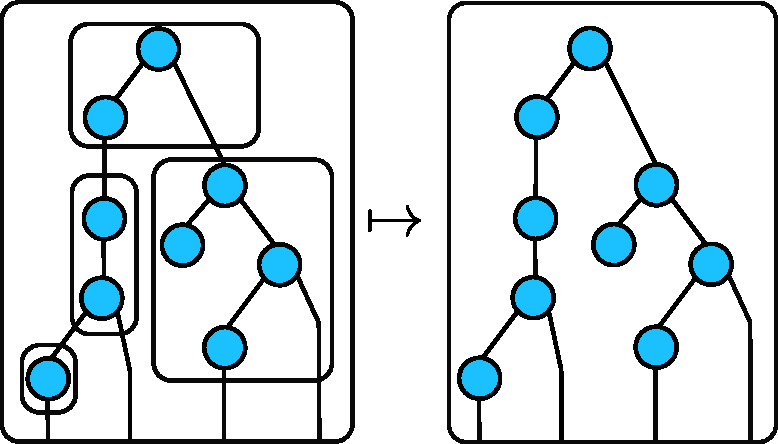
\includegraphics[scale=0.33]{flat}}
\end{array} \quad&\quad \begin{array}{cc}
\simplefun
        {}
        {\Sigma}
        {\reduce 1 \Sigma}
        {
        
\includegraphics[scale=0.33]{g-unit}}
        & 
        \simplefun
        {}
        {\reduce k \reduce l \Sigma}
        {\reduce{k.l} \Sigma} 
        {  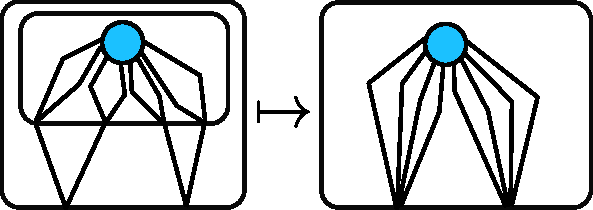
\includegraphics[scale=0.33]{g-flat}}
\end{array}
\end{array}$\\[15pt]


$
\begin{array}{c}
  \textbf{Accociativity} \\[5pt]
\begin{array}{ccc}
	\simplefun
        {}
        {(\Sigma \otimes \Gamma)\otimes \Delta}
        {\Sigma \otimes (\Gamma\otimes \Delta)}
        {$\tensorpair{\tensorpair{a,b},c}\mapsto \tensorpair{a,\tensorpair{b,c}}$} 	
 	& \simplefun
        {}
        {(\Sigma + \Gamma)+ \Delta }
        { \Sigma + (\Gamma+ \Delta)}
        {$\begin{array}{lll}
        ((a,1),1)& \to &(a,1)\\
         ((a,2),1)& \to & ((a,1),2)\\
         (a,2) & \to & ((a,2),2)
        \end{array}$} 	
 	&  \simplefun
        {}
        {(\Sigma \cdot \Gamma)\cdot \Delta }
        { \Sigma \cdot (\Gamma \cdot \Delta)}
        {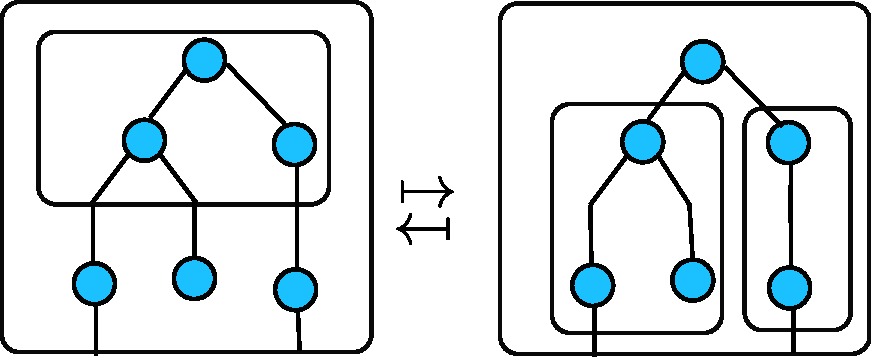
\includegraphics[scale=.3]{associativity-shallow}} 
\end{array} 
\\[15pt]
 \textbf{Distributivity} \\[5pt]
\begin{array}{ccc}
\reversiblefun
        {}
        {\shallowterm {(\Sigma_1 + \Sigma_2)} \Gamma}
        {(\shallowterm {\Sigma_1} \Gamma) + (\shallowterm {\Sigma_2} \Gamma)}
        {$(a,i)\tensorpair{t_1,\dots,t_n} \to (a\tensorpair{t_1,\dots,t_n},i)$}
        &
        \reversiblefun
        {}
        {(\Sigma_1 + \Sigma_2)\otimes \Gamma}
        {(\Sigma_1 \otimes \Gamma) + (\Sigma_2 \otimes \Gamma)}
        {$\tensorpair{(a,i),b}\to (\tensorpair{a,b},i)$}
        &       
        \simplefun
        {}
        {\reduce k (\Sigma_1 + \Sigma_2)}
        {\reduce k \Sigma_1 + \reduce k \Sigma_2}
         {$(a,i)/f \mapsto ((a/f),i)$}
      \\[15pt]  
      \reversiblefun
        {}
        {\shallowterm {(\Sigma_1 \otimes \Sigma_2)} \Gamma}
        {(\shallowterm {\Sigma_1} \Gamma) \otimes (\shallowterm {\Sigma_2} \Gamma)}
        {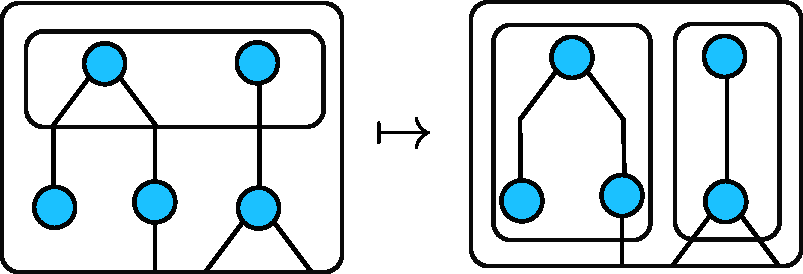
\includegraphics[scale=.33]{tensor-shallow-distrib}}
%        {(a,i)\tensorpair{b_1,\ldots,b_n} \mapsto (a\tensorpair{b_1\ldots,b_n}) }
%       &
%        {\tensorpair{(a,i),b} \mapsto (\tensorpair{a,b},i)}
%       &
%        {
%        \begin{tabular}{c}
%            $\tensorpair{a_1,a_2}\tensorpair{b_1,\ldots,b_n} \mapsto$ \\
%            $\tensorpair{a_1 \tensorpair{b_1,\ldots,b_{n_1}}, a_2\tensorpair{b_{n_1+1},\ldots,b_n} }$  \\
%            where $n_1$ is the arity of $a_1$
%            \end{tabular}}                
         & 
	\simplefun
        {}
        {\reduce k (\Sigma_1 \otimes \Sigma_2)}
        {\reduce k ((\reduce k {\Sigma_1})\otimes (\reduce k \Sigma_2))}
        {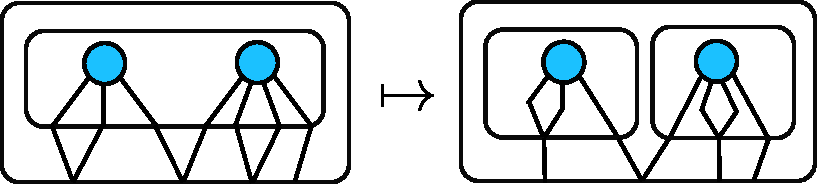
\includegraphics[scale=.33]{tensor-fold-distrib-1}}        
	&
	 \simplefun
        {}
        {(\reduce k \Sigma_1) \otimes (\reduce k {\Sigma_2})}
         {\reduce k (\Sigma_1 \otimes \Sigma_2)}
        {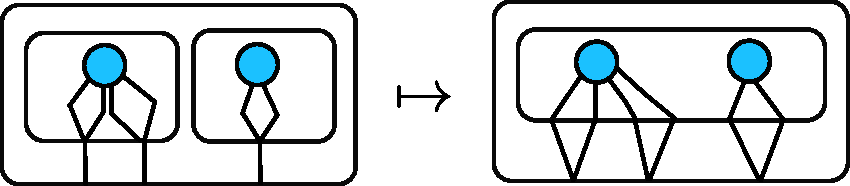
\includegraphics[scale=.33]{tensor-fold-distrib-2}}  
         \end{array}\\
\begin{array}{cc}
  \simplefun
        {}
        {\shallowterm \Sigma {\reduce k \Gamma}}
         {\reduce k (\shallowterm \Sigma {\Gamma})}{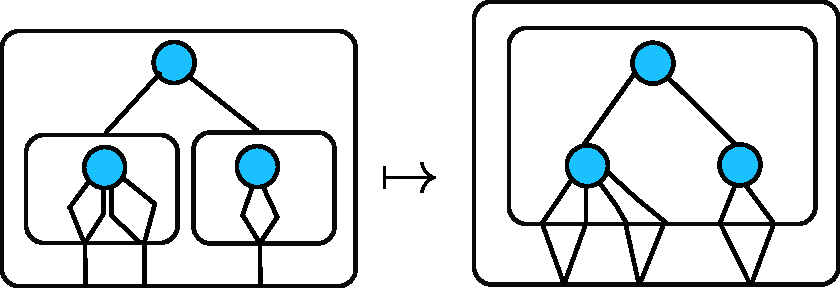
\includegraphics[scale=.33]{shallow-fold-distrib}} &        
         \simplefun
        {}
        {\tmonad {\reduce 1\Sigma}}
         {\reduce 1 \tmonad \Sigma}
         {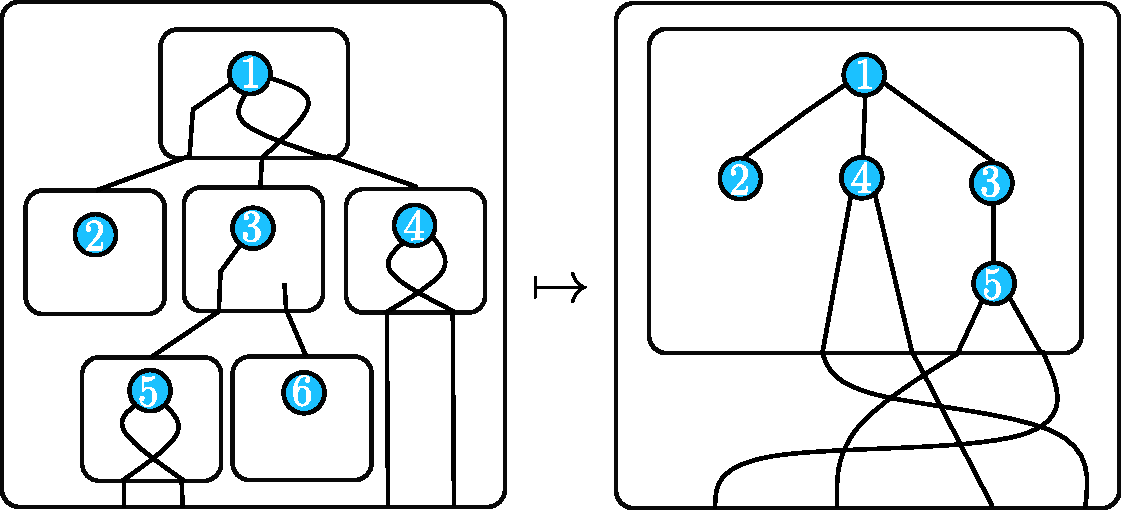
\includegraphics[scale=.33]{unfold-1}}
\end{array}   
         \end{array}
$\\[15pt]

$
\begin{array}{c}
\textbf{Injections}\\[5pt]
\begin{array}{cccc}
	\simplefun
        {\iota_i}
        {\Sigma}
        {\Sigma+\Sigma}
        {$a \mapsto (a,i)$}		
	& \simplefun
        {}
        {\Sigma}
        { \reduce k \Sigma^k}
        {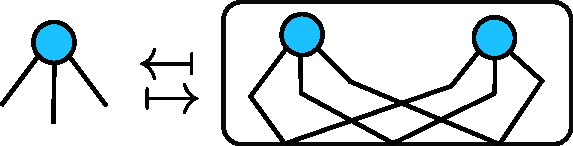
\includegraphics[scale=.3]{tensor-injection}}	 
	&
	\simplefun
        {}
        {\reduce k \Sigma}
        { \reduce {k+1}\Sigma}
        {
\includegraphics[scale=.3]{add-fold}}	 
	&\simplefun
        {}
        {\Sigma^n}
        { \shallowterm n \Sigma}
        {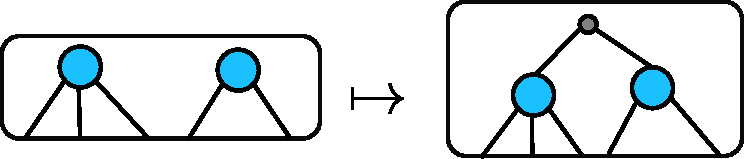
\includegraphics[scale=.3]{tensor-injection-2}}	
\end{array} \\[15pt]
\textbf{Projections}\\[5pt]
\begin{array}{cccc}
	\simplefun
        {}
        {\Sigma+\Sigma}
        {\Sigma}
        {$(a,i)\to a$}	
	& \simplefun
        {}
        {\Sigma\otimes \Sigma}
        {\reduce 1 \Sigma}
        {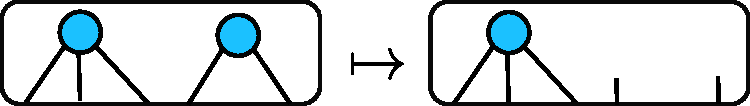
\includegraphics[scale=.3]{tensor-projection-1}}	 
	& \simplefun
        {}
        {\reduce {k+1} \Sigma}
        {\reduce {k}\Sigma+\bot}
        {
\includegraphics[scale=.3]{reduce-fold}}	 
	& \simplefun
        {}
        {\shallowterm n \Sigma }
        {\Sigma^n}
        {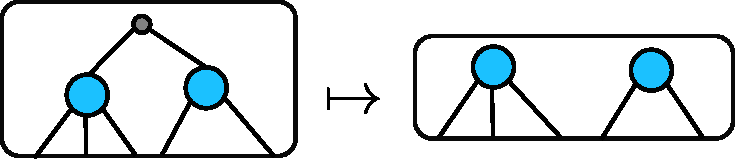
\includegraphics[scale=.3]{tensor-projection-2}}	
\end{array}
\end{array}
$\\[15pt]

$
\begin{array}{cc}
\textbf{Commutativity} & \textbf{Shallow terms} \\
\begin{array}{cc}
      \reversiblefun
        {}
        {\ranked{\Sigma_1 + \Sigma_2}}
        {\ranked{\Sigma_2 + \Sigma_1}}
        {$(a,i) \mapsto (a,3-i) $}
  &
    \reversiblefun
        {}
        {\ranked{\Sigma_1 \otimes\Sigma_2}}
        {\ranked{\Sigma_2 \otimes \Sigma_1}}
        {$\tensorpair{a,b} \mapsto \tensorpair{b,a} $}
\end{array}\qquad&\qquad
\begin{array}{cc}
  \reversiblefun
        {}
        {\rSigma}
        {\shallowterm {\Sigma} 1}
        {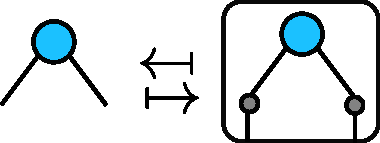
\includegraphics[scale=.3]{sigma-dot-1}}
      &
        \reversiblefun
        {\composeterm}
        {1 + \shallowterm \Sigma {\tmonad \Sigma} }
        { \tmonad \Sigma}
        {
        \begin{tabular}{l}
            Every term is either just a port,\\ or has a root and child subterms.    
        \end{tabular}    
        }
\end{array}
\end{array}
$\\[15pt]


$\begin{array}{c}
        \textbf{Functions explained in Section~\ref{sec:prime-and-combinators}}   \\[5pt]
\begin{array}{cccc}
\begin{tabular}{cc}
        $\ranked{
        \xymatrix@C=1cm{
\tmonad(\Sigma_1+\Sigma_2) \ar@<.5ex>[r]^{ \ancfact}
        \ar@<-.5ex>[r]_{\decfact}& \tmonad(\tmonad \Sigma_1 + \tmonad \Sigma_2)
        }}$
        \end{tabular} 
                  &
      \begin{tabular}{cc}
        $\ranked{
        \xymatrix@C=.7cm{
\tmonad \Sigma \ar[r]^-{\preorder}& \reduce 1 \tmonad(\rSigma + 0 + 2)
        }}$
    \end{tabular}
        &
       \begin{tabular}{cc}
        $\ranked{
        \xymatrix@C=.7cm{
\shallowterm{(\reduce k \Sigma)}{\Gamma^k} \ar[r]^-{\unfold}& \reduce 1(\shallowterm \Sigma \Gamma)
        }}$
    \end{tabular}
    &
      \begin{tabular}{cc}
        $\ranked{
        \xymatrix@C=.9cm{
\tmonad {\reduce k \Sigma} \ar[r]^-{\text{external}}_{\text{unfold}\ }& \reduce k \tmonad \reduce k \Sigma
        }}$
    \end{tabular}
\end{array}   
\end{array}$
\caption{    \label{fig:fo-term}The prime functions. The functions are parametrised by types  $\rSigma, \ranked{\Sigma_1}, \ranked{\Sigma_2}, \rGamma$. Some of the functions are bijections, as indicated by double arrows, in these cases both the function and its inverse are prime functions. }
\end{figure*}



%
%
%\newpage
%\begin{enumerate}
%\item \textbf{The monad $\tmonad$.}
%$$\begin{array}{ll}
%  \simplefun
%        {\unit_\Sigma}
%        {\Sigma}
%        {\tmonad \Sigma}
%        {
%      \includegraphics[page=10,scale=0.4]{pics}}
%        & 
%        \simplefun
%        {\flatt_\Sigma}
%        {\tmonad \tmonad \Sigma}
%        {\tmonad \Sigma} 
%        {\tablepic{73}}
%\end{array}$$
%\item \textbf{The graded monad $\reduce k$.}
%$$\begin{array}{ll}
%  \simplefun
%        {}
%        {\Sigma}
%        {\reduce 1 \Sigma^1}
%        {} &
%        \simplefun
%        {}
%        {\reduce {k_1} \reduce {k_2} \Sigma}
%        {\reduce {k_1 \cdot k_2} \Sigma}
%        {$(a/f)/g \mapsto a/(g \circ f)$}
%        \end{array}$$
%\item \textbf{Associativity functions.}
%$$\begin{array}{lll}
%\ranked{(\Sigma \otimes \Gamma)\otimes \Delta \to \Sigma \otimes (\Gamma\otimes \Delta)} \quad &\quad \ranked{(\Sigma + \Gamma)+ \Delta \to \Sigma + (\Gamma+ \Delta)}  \quad&\quad \ranked{(\Sigma . \Gamma). \Delta \to \Sigma . (\Gamma . \Delta)}
%\end{array}$$
%\item \textbf{Distributivity functions}.
%$$\begin{array}{ll}
%      \simplefun
%        {}
%        {\reduce k (\Sigma_1 + \Sigma_2)}
%        {\reduce k \Sigma_1 + \reduce k \Sigma_2}
%        {$(a,i)/f \mapsto ((a/f),i)$}
%         & 
%        \reversiblefun
%        {}
%        {(\Sigma_1 + \Sigma_2)\otimes \Gamma}
%        {(\Sigma_1 \otimes \Gamma) + (\Sigma_2 \otimes \Gamma)}
%        {$\tensorpair{(a,i),b} \mapsto (\tensorpair{a,b},i)$}
%        \\ \\
%        \reversiblefun
%        {}
%        {\shallowterm {(\Sigma_1 + \Sigma_2)} \Gamma}
%        {(\shallowterm {\Sigma_1} \Gamma) + (\shallowterm {\Sigma_2} \Gamma)}
%        {$(a,i)\tensorpair{b_1,\ldots,b_n} \mapsto (a\tensorpair{b_1,\ldots,b_n})$ }
%        &
%        \reversiblefun
%        {}
%        {\shallowterm {(\Sigma_1 \otimes \Sigma_2)} \Gamma}
%        {(\shallowterm {\Sigma_1} \Gamma) \otimes (\shallowterm {\Sigma_2} \Gamma)}
%        {
%        \begin{tabular}{c}
%            $\tensorpair{a_1,a_2}\tensorpair{b_1,\ldots,b_n} \mapsto$ \\
%            $\tensorpair{a_1 \tensorpair{b_1,\ldots,b_{n_1}}, a_2\tensorpair{b_{n_1+1},\ldots,b_n} }$  \\
%            where $n_1$ is the arity of $a_1$
%            \end{tabular}}
%            \\
%	\simplefun
%        {}
%        {\reduce k (\Sigma_1 \otimes \Sigma_2)}
%        {\reduce k ((\reduce k {\Sigma_1})\otimes (\reduce k \Sigma_2))}{picture}        
%	&
%	 \simplefun
%        {}
%        {(\reduce k \Sigma_1) \otimes (\reduce k {\Sigma_2})}
%         {\reduce k (\Sigma_1 \otimes \Sigma_2)}
%        {picture}  \\
%        
%         \simplefun
%        {}
%        {\shallowterm \Sigma {\reduce k \Gamma}}
%         {\reduce k (\shallowterm \Sigma {\Gamma})}
%        
%&        
%\end{array} $$
%\item \textbf{Commutativity functions.} 
%$$\begin{array}{ll}
%\ranked{\Sigma_1 + \Sigma_2 \to \Sigma_2 + \Sigma_1} \qquad & \qquad  \ranked{\Sigma_1 \otimes \Sigma_2 \to \Sigma_2 \otimes \Sigma_1}
%\end{array}
%$$
%\item \textbf{Shallow terms.} 
%   $$\begin{array}{lll}
%   \reversiblefun
%        {}
%        {\rSigma}
%        {\shallowterm 1 {\Sigma} }
%        {picture}
%        &
%      \reversiblefun
%        {}
%        {\rSigma}
%        {\shallowterm {\Sigma} 1}
%        {picture}
%        &
%        \reversiblefun
%        {\composeterm}
%        {1 + \shallowterm \Sigma {\tmonad \Sigma} }
%        { \tmonad \Sigma}
%        {
%        \begin{tabular}{c}
%            Every term is either just a port,\\ or has a root and child subterms.    
%        \end{tabular}    
%        } 
%\end{array} $$     
%\item \textbf{The error type $\bot$.} Some error raising mechanisms.
%$$\begin{array}{llll}
%\ranked{\Sigma \to \bot} \quad&\quad \ranked{\tmonad(\Sigma+\bot)\to \tmonad\Sigma+\bot} \quad&\quad \ranked{\reduce k (\Sigma+\bot)\to \reduce k\Sigma+\bot}\quad&\quad  \ranked{(\Sigma+\bot)\otimes \Gamma\to \Sigma\otimes \Gamma+\bot}
%\end{array}$$     
%\item \textbf{Injections.}
%$$\begin{array}{llll}
%\ranked{\Sigma \to \Sigma+\Sigma} \quad &\quad \ranked{\Sigma \to \reduce k \Sigma^k}  \quad & \quad \ranked{\reduce k \Sigma \to \reduce {k+l}\Sigma} \quad & \quad 
%\ranked{\Sigma^n\to  \shallowterm n \Sigma}
%\end{array}$$
%\item \textbf{Projections.}
%$$\begin{array}{llll}
%\ranked{\Sigma+\Sigma\to \Sigma} \quad &\quad \ranked{\Sigma\otimes \Sigma \to \reduce 1 \Sigma} \quad & \quad \ranked{\reduce {k+1} \Sigma \to \reduce {k}\Sigma+\bot} \quad & \quad 
%\ranked{\shallowterm n \Sigma \to \Sigma^n} 
%\end{array}$$
%\item \textbf{Factorisations.} Same as before.
%\item \textbf{Pre-order.} Same as before.
%\item \textbf{Unfolding.} We have 3 unfolding functions. The first is the shallow unfold, the second is 
%\begin{align*}
%\ranked{\tmonad \reduce 1 \Sigma \to \reduce 1 \tmonad \Sigma }
%\end{align*}
%The third is \emph{the unfolding of external twists}. This function, which is of type 
%\begin{align*}
%\ranked{\tmonad \mati k \Sigma \to \reduce k \tmonad \mati k \Sigma}
%\end{align*}
%"untwists" the external twists  as illustrated by the following figure where the external twists have been colored in red. 
%\begin{center}
%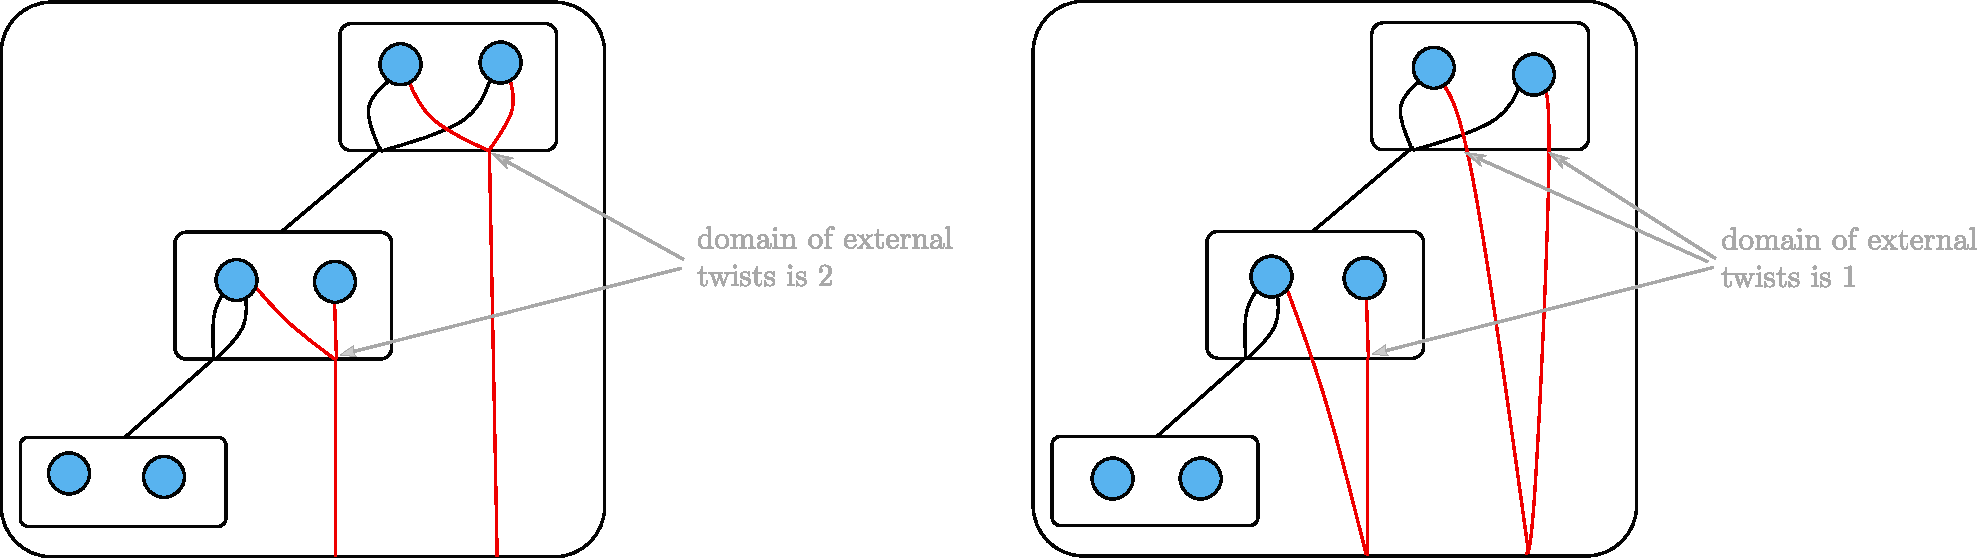
\includegraphics[scale=.4]{external-unfold.pdf}
%\end{center}
%\end{enumerate}
%
